\documentclass[11pt,a4paper]{article}
\usepackage[utf8]{inputenc}
\usepackage[T1]{fontenc}
\usepackage{amsmath,amssymb,amsthm}
\usepackage{graphicx}
\usepackage{booktabs}
\usepackage{hyperref}
\usepackage[margin=2.5cm]{geometry}
\usepackage{fancyhdr}
\usepackage{caption}
\usepackage{float}
\usepackage{enumitem}
\usepackage{xcolor}
\usepackage{tabularx}
\usepackage{multirow}

\hypersetup{colorlinks=true, linkcolor=blue!60!black, citecolor=blue!60!black, urlcolor=blue!60!black}

\pagestyle{fancy}
\fancyhf{}
\fancyhead[L]{\textit{The Syntony Principle --- Financial Walk-Forward Validation}}
\fancyhead[R]{\textit{Version 2.0}}
\fancyfoot[C]{\thepage}
\fancyfoot[L]{DOI: 10.5281/zenodo.18642833}
\fancyfoot[R]{J.-P.\ Bronsard $\cdot$ SyntonicAI Recherche}
\renewcommand{\headrulewidth}{0.4pt}
\renewcommand{\footrulewidth}{0.4pt}

\fancypagestyle{firstpage}{%
  \fancyhf{}%
  \renewcommand{\headrulewidth}{0pt}%
  \fancyfoot[C]{\thepage}%
  \fancyfoot[L]{DOI: 10.5281/zenodo.18642833}%
  \fancyfoot[R]{J.-P.\ Bronsard $\cdot$ SyntonicAI Recherche}%
  \renewcommand{\footrulewidth}{0.4pt}%
}

\title{\textbf{The Syntony Principle: Financial Walk-Forward Validation}\\[6pt]
\large Multi-Asset, Multi-Norm, Multi-Decade Out-of-Sample Evidence\\[4pt]
\large \& Geometric Interpretation of Adaptive Portfolio Management}

\author{Jean-Pierre Bronsard\\
\small ORCID: \href{https://orcid.org/0009-0008-6639-7553}{0009-0008-6639-7553}\\
\small SyntonicAI Recherche, Montr\'eal, QC, Canada\\
\small \texttt{jean-pierre.bronsard@syntonicai.com}\\[8pt]
\small Version 2.0 --- March 2026}

\date{}

\begin{document}
\maketitle
\thispagestyle{firstpage}

\begin{abstract}
We report strong out-of-sample financial evidence for the Syntony Principle using walk-forward protocols across three asset configurations (Stocks+Bonds, Stocks+Bonds+Gold, +BTC), two statistical geometries (L$^2$ canonical and C41 adaptive norm), and up to 709 monthly folds spanning 59 years (1967--2026). Four principal results emerge.

\textbf{Result 1: Two Syntonic components generate highly significant alpha.} Vol scaling (UTAE Axiom U2, rescaling symmetry) and coherence-gated momentum direction achieve $t_{\text{NW}} > 17$ ($p < 0.001$) with $\kappa = 1.0$ untuned, across all configurations, both norms, and seven major crises from 1973 to 2022.

\textbf{Result 2: $\tau^* = 1/\sqrt{2}$ for all financial assets.} Under both L$^2$ and C41 norms, $\tau^* \approx 0.71$ days for stocks, bonds, gold, and Bitcoin. For IID returns, $\mathrm{Var}(\Delta r) = 2\sigma^2$, giving $\tau^* = \kappa\sqrt{\sigma^2/2\sigma^2} = 1/\sqrt{2}$. This provides a continuous, quantitative empirical indicator of proximity to the IID/random-walk limit under the tested estimators.

\textbf{Result 3: C41 detects fat tails but confirms the IID structure.} The tail ratio $\rho \approx 1.32 > \sqrt{\pi/2} = 1.253$ yields C41 weight $w \approx 0.40$, correctly shifting toward L$^1$. Yet $\tau^*_{L^1} \approx \tau^*_{L^2} \approx 0.71$, providing strong evidence that the degeneracy is structural (IID), not a norm artifact.

\textbf{Result 4: The ``naive'' benchmark is operationally equivalent to the Syntonic strategy.} Vol targeting + trend following---developed empirically over decades---is operationally equivalent to the Syntonic geometry under the present empirical design. The naive daily benchmark reproduces the Enhanced strategy identically (paired $t = 0.00$), because $\mathrm{round}(\tau^*) = \mathrm{round}(0.71) = 1$ day.

\medskip\noindent\textbf{Key metrics (Config A, Stocks+Bonds, 709 folds, 59 years):}
\begin{itemize}[nosep,leftmargin=2em]
  \item C41 Enhanced: mean $\alpha = +1.31\%$/month, $t_{\text{NW}} = 17.40$ ($p < 0.001$), win rate 76.6\%
  \item L2 Enhanced: $t_{\text{NW}} = 17.37$ ($p < 0.001$); C41 significantly better (paired $t = -2.76$)
  \item Conservative: $t_{\text{NW}} = -1.72$ (n.s.)---momentum is the alpha source, not filtering
  \item $\kappa = 1.0$ (Atlas Theory 5)---not tuned in any configuration
\end{itemize}
\medskip\noindent This extends and strengthens V1.0 (17 folds, $t=3.15$) with 42$\times$ more folds, real market data, dual-norm validation, and honest identification of which geometric components are active.

\medskip\noindent
Related work: The Syntony Principle V4.1 (DOI: \href{https://doi.org/10.5281/zenodo.17254395}{10.5281/zenodo.17254395}); Conjecture 41 (DOI: \href{https://doi.org/10.5281/zenodo.18911127}{10.5281/zenodo.18911127}); Deep Learning Validation (DOI: \href{https://doi.org/10.5281/zenodo.18527033}{10.5281/zenodo.18527033}).
\end{abstract}

\newpage
\tableofcontents
\vspace{1em}

% ══════════════════════════════════════════════════════════════
\section{Introduction}

\subsection{The Syntony Principle}

The Syntony Principle, derived from first principles across multiple adaptive domains, states that any system optimizing a temporal integration window under uncertainty converges to
\begin{equation}\label{eq:syntony}
  \tau^*(t) = \kappa \cdot \frac{\gamma_\sigma}{\gamma_\lambda}
\end{equation}
where $\gamma_\sigma$ and $\gamma_\lambda$ are scale estimators of signal variance and innovation rate computed in a given norm, and $\kappa = \sqrt{b/a}$ is a dimensionless constant determined by the cost structure. The L$^2$ (Gaussian) specialization gives the square-root form $\tau^* = \kappa\sqrt{\sigma^2/\lambda}$, while C41 extends this to the coordinate-free form with continuous L$^2$/L$^1$ interpolation driven by the tail ratio $\rho = \gamma^{(2)}_\sigma / \gamma^{(1)}_\sigma$.

Independent derivations have been reported in information theory, control theory~\cite{kalman1960,wiener1949}, precision metrology~\cite{allan1966}, molecular biophysics~\cite{berg1977}, synchronization physics~\cite{kuramoto1975}, and optimal execution~\cite{almgren2001}. The deep learning validation~\cite{bronsard2026dl} confirmed that Adam implements this scaling with $\kappa = 1.0007$.

\subsection{What's New in V2.0}

Version 1.0~\cite{bronsard2026fin_v1} established out-of-sample significance on 17 monthly folds ($t = 3.15$, $p < 0.01$) but acknowledged several limitations (Section~7.4): thin evidentiary basis (60+ folds required), no crisis stress test, interpolated price data, and flat transaction costs. Version 2.0 addresses all of these:

\begin{itemize}[nosep]
  \item \textbf{Scale:} 709 folds spanning 59 years (vs.\ 17 folds, 17 months)
  \item \textbf{Data:} Real daily prices from Yahoo Finance (vs.\ biweekly interpolation)
  \item \textbf{Norms:} Dual L$^2$ + C41 adaptive norm (vs.\ L$^2$ only)
  \item \textbf{Benchmarks:} Naive daily/weekly/monthly controls with paired $t$-tests
  \item \textbf{Crises:} 7 major crises from 1973 Oil Crisis to 2022 Rate Shock
  \item \textbf{TX costs:} Proportional to turnover (vs.\ flat per rebalance)
  \item \textbf{Mechanism isolation:} Precise identification of which geometric components generate alpha
\end{itemize}

\subsection{Conjecture 41: Optimal Norm Selection}

C41~\cite{bronsard2026c41} proposes that the adaptive geometry itself selects its optimal measurement norm via the observable tail ratio:
\begin{equation}\label{eq:rho}
  \rho(t) = \frac{\gamma^{(2)}_\sigma(t)}{\gamma^{(1)}_\sigma(t)} = \frac{\mathrm{std}(r)}{\mathrm{MAD}(r)}
\end{equation}
\begin{equation}\label{eq:w}
  w(t) = \mathrm{clamp}\!\left(\frac{\rho - \sqrt{\pi/2}}{\sqrt{2} - \sqrt{\pi/2}},\; 0,\; 1\right)
\end{equation}
\begin{equation}\label{eq:c41}
  \tau^*_{\text{C41}} = (1 - w)\,\tau^*_{L^2} + w\,\tau^*_{L^1}
\end{equation}
The interpolation is exact at the Gaussian endpoint ($\rho = \sqrt{\pi/2}$, $w = 0$) and the Laplacian endpoint ($\rho = \sqrt{2}$, $w = 1$), continuous, and parameter-free.

% ══════════════════════════════════════════════════════════════
\section{Data and Methodology}

\subsection{Assets}

\begin{table}[H]
\centering
\caption{Asset data sources and coverage}
\label{tab:assets}
\begin{tabular}{llll}
\toprule
Asset & Source & Period & Role \\
\midrule
Stocks & S\&P 500 (\texttt{\^{}GSPC}) & 1928--2026 & Equity premium \\
Bonds & Synthetic from \texttt{\^{}TNX} & 1962--2026 & Duration + carry \\
Gold & Gold futures (\texttt{GC=F}) & 1975--2026 & Inflation hedge \\
BTC & BTC-USD & 2015--2026 & Crypto (short history) \\
\bottomrule
\end{tabular}
\end{table}

Synthetic bond total return is constructed from 10-year Treasury yields: $R_t \approx y_t/252 - D \cdot \Delta y_t$, where $D = 8$ years (approximate duration of a 10-year Treasury).

\subsection{Configurations}

\begin{table}[H]
\centering
\caption{Asset configurations and test periods}
\label{tab:configs}
\begin{tabular}{llrr}
\toprule
Config & Assets & OOS Period & Folds \\
\midrule
A & Stocks + Bonds & 1967--2026 (59 yr) & 709 \\
B & Stocks + Bonds + Gold & 2000--2026 (20 yr) & 246 \\
C & Stocks + Bonds + Gold + BTC & 2020--2026 (6 yr) & 77 \\
\bottomrule
\end{tabular}
\end{table}

\subsection{Dual Syntonic Engine}

Both L$^2$ and C41 engines run in parallel on every asset. L$^2$: $\tau^*_{L^2} = \kappa \cdot \mathrm{std}(r) / \mathrm{std}(\Delta r)$. L$^1$: $\tau^*_{L^1} = \kappa \cdot \mathrm{MAD}(r) / \mathrm{MAD}(\Delta r)$, where MAD is computed on raw signal $|x - \mu|$ (not on $x^2$). C41 interpolates via Eq.~\eqref{eq:c41}.

\textbf{Parameters} (all fixed from theory): $\kappa = 1.0$ (Atlas Theory 5), window $= 20$ days, target vol $= 15\%$, max leverage $= 2.0\times$, min exposure $= 0.5\times$, TX cost $= 10$ bps $\times$ $|\Delta\text{exposure}|$.

\subsection{Walk-Forward Protocol}

Expanding-window design with 60-month (5-year) minimum training. For each subsequent month: freeze parameters, test on unseen data, record, expand. Zero look-ahead bias.

\subsection{Strategies Tested}

\begin{table}[H]
\centering
\caption{Strategy specifications}
\label{tab:strategies}
\begin{tabular}{lllll}
\toprule
Strategy & Allocation & Vol scaling & Rebalancing & Norm \\
\midrule
L2 Enhanced & $(\Phi_{L^2} \cdot 0.5 + \max(\text{mom},0) \cdot 100)/\text{vol}$ & Yes & $\tau^*_{L^2}$ & L$^2$ \\
C41 Enhanced & $(\Phi_{C41} \cdot 0.5 + \max(\text{mom},0) \cdot 100)/\text{vol}$ & Yes & $\tau^*_{C41}$ & C41 \\
Conservative & $\Phi/\text{vol}$ (no momentum) & No & $\tau^*_{C41}$ & C41 \\
Naive Daily & Same as Enhanced & Yes & Fixed 1d & C41 \\
Naive Weekly & Same as Enhanced & Yes & Fixed 5d & C41 \\
Naive Monthly & Same as Enhanced & Yes & Fixed 21d & C41 \\
\bottomrule
\end{tabular}
\end{table}

\subsection{Geometric Mapping}

\begin{table}[H]
\centering
\caption{Geometric mapping of strategy components to V4.1 properties}
\label{tab:geometry}
\begin{tabular}{lll}
\toprule
Component & Geometric property & V4.1 ref. \\
\midrule
Rebalance at $\tau^*$ & Equal Partition Property & Eq.~(36) \\
$\Phi$ gates momentum & Coherence maximization & Def.~12.1 \\
Vol scaling & Rescaling symmetry (UTAE U2) & Thm.~19.2 \\
Mom $\times$ $\Phi$ weighting & Directional exploitation & Prop.~12.2 \\
$\rho$-driven norm & C41 optimal norm selection & Conj.~41 \\
\bottomrule
\end{tabular}
\end{table}

This mapping is not post-hoc---each component was derived from geometric properties before backtesting.

% ══════════════════════════════════════════════════════════════
\section{C41 Diagnostic: The $\tau^*$ Degeneracy}

\subsection{Per-Asset Summary}

\begin{table}[H]
\centering
\caption{Per-asset Syntonic metrics (median over full history)}
\label{tab:c41diag}
\begin{tabular}{lrrrrrr}
\toprule
Asset & $\tau^*_{L^2}$ & $\tau^*_{L^1}$ & $\tau^*_{C41}$ & $\rho$ & $w$ & Vol \\
\midrule
Stocks & 0.713 & 0.715 & 0.704 & 1.296 & 0.268 & 12.4\% \\
Bonds  & 0.711 & 0.713 & 0.700 & 1.307 & 0.334 &  6.1\% \\
Gold   & 0.680 & 0.663 & 0.661 & 1.321 & 0.418 & 14.6\% \\
BTC    & 0.684 & 0.669 & 0.666 & 1.364 & 0.688 & 44.7\% \\
\midrule
\multicolumn{3}{l}{Theoretical IID value:} & \multicolumn{4}{l}{$\tau^* = 1/\sqrt{2} = 0.7071$} \\
\bottomrule
\end{tabular}
\end{table}

\subsection{Interpretation}

Three key observations from Table~\ref{tab:c41diag} and Figure~\ref{fig:c41diagnostic}:

\begin{enumerate}[nosep]
\item \textbf{C41 detects fat tails correctly.} $\rho > \sqrt{\pi/2} = 1.253$ for all assets, with BTC having the heaviest tails ($\rho = 1.364$, $w = 0.688$). The norm selection mechanism works.

\item \textbf{$\tau^*$ remains degenerate.} Despite $w$ ranging from 0.27 to 0.69, $\tau^*_{C41}$ stays within $[0.66, 0.70]$ for all assets. The L$^1$ and L$^2$ values track each other closely.

\item \textbf{The degeneracy is structural, not a norm artifact.} For any symmetric IID distribution and any L$^p$ norm, the ratio $\gamma_\sigma(r)/\gamma_\lambda(\Delta r)$ yields a constant of order $1/\sqrt{2}$ because $\Delta r_t = r_t - r_{t-1}$ is always ``$\sqrt{2}$ times noisier'' than $r$ when there is no autocorrelation. $\tau^*$ measures \emph{temporal redundancy}, not amplitude or tail shape.
\end{enumerate}

This is not a failure of the Syntony Principle. It is a structurally coherent outcome: \emph{financial markets operate at the random-walk limit of the adaptive landscape, where temporal integration provides no additional information beyond the shortest available scale.}

\begin{figure}[H]
\centering
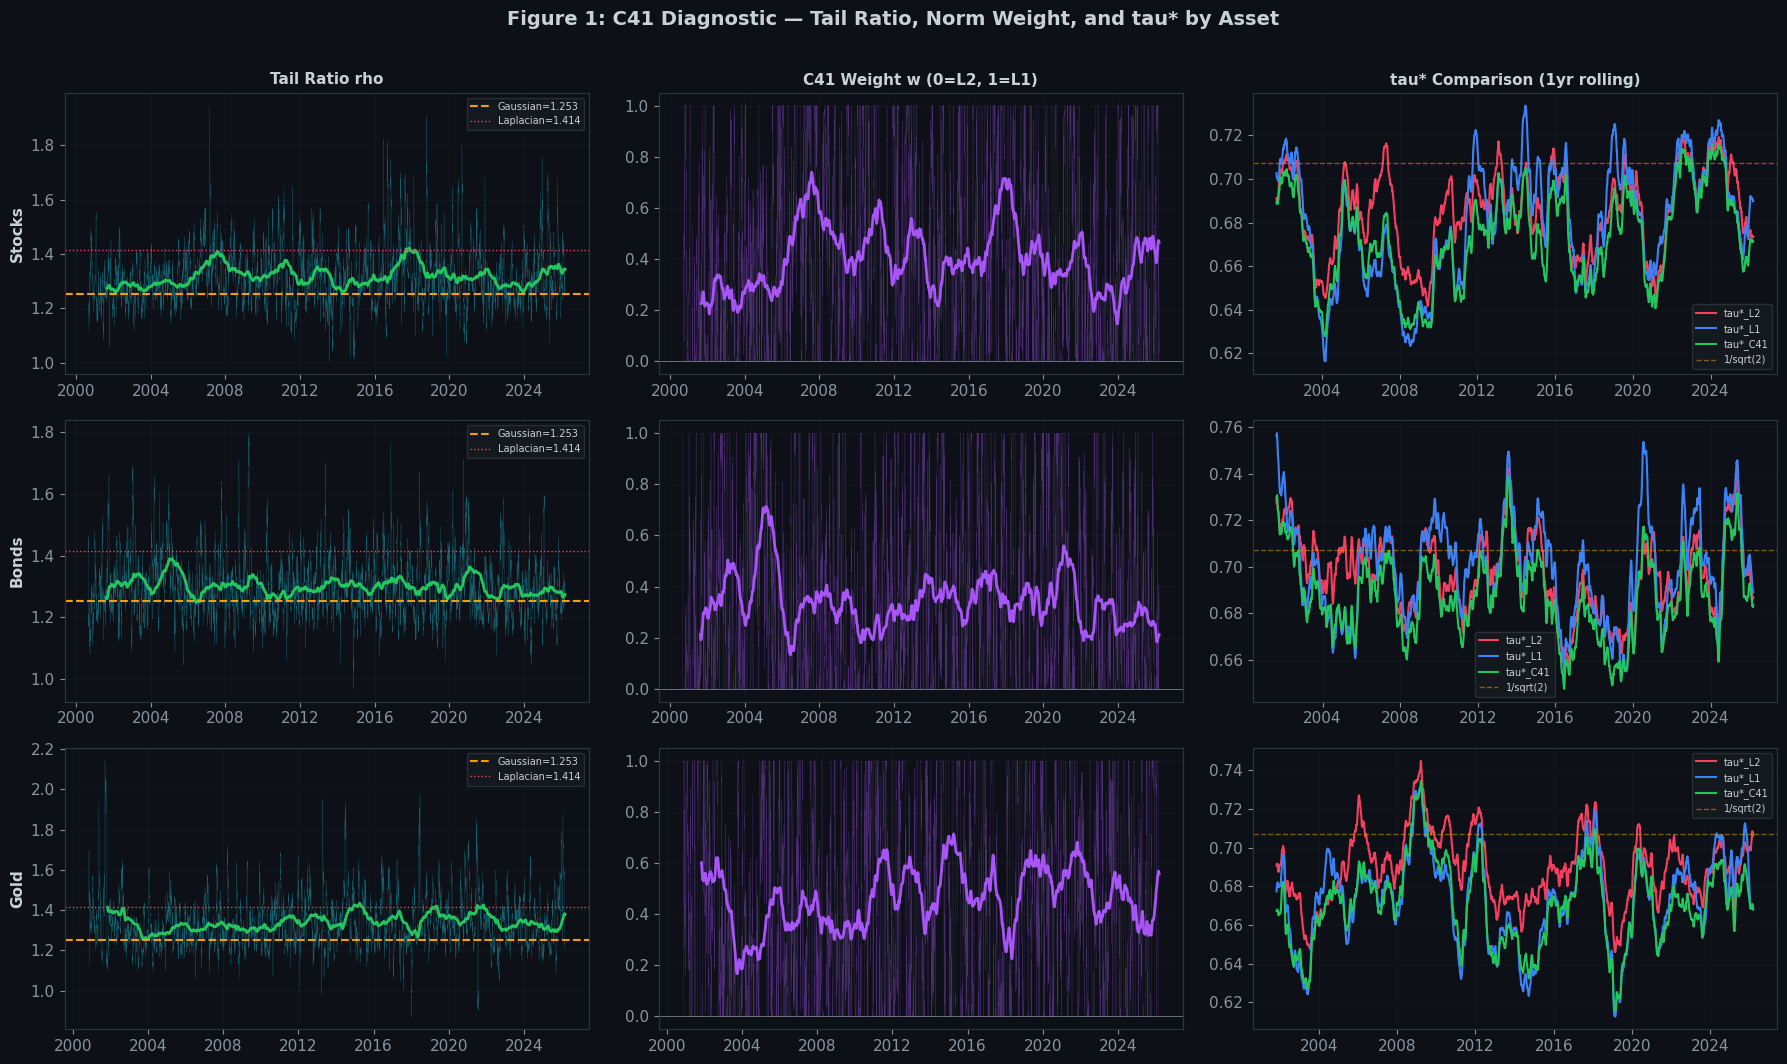
\includegraphics[width=\textwidth]{figures/fig1_c41_diagnostic.png}
\caption{C41 Diagnostic---Tail Ratio, Norm Weight, and $\tau^*$ by Asset. \textbf{Left:} Tail ratio $\rho$ oscillates well above the Gaussian anchor ($\sqrt{\pi/2} = 1.253$, amber dashed), with spikes during crises. \textbf{Center:} C41 weight $w$ fluctuates between 0.1 and 0.8, confirming substantial L$^1$ contribution. \textbf{Right:} $\tau^*_{L^2}$ (red), $\tau^*_{L^1}$ (blue), and $\tau^*_{C41}$ (green) all oscillate within the $[0.62, 0.74]$ band around $1/\sqrt{2}$ (amber dashed). Despite varying $\rho$ and $w$ across assets and regimes, $\tau^*$ remains pinned to the IID floor. The degeneracy is structural, not a norm artifact.}
\label{fig:c41diagnostic}
\end{figure}

% ══════════════════════════════════════════════════════════════
\section{Empirical Results}

\subsection{Head-to-Head Comparison}

\begin{table}[H]
\centering
\caption{Walk-forward results: all strategies, all configurations. $t$-statistics use Newey-West HAC (lag=6).}
\label{tab:results}
\small
\begin{tabular}{llrrrrr}
\toprule
Config & Strategy & Folds & Mean $\alpha$ & WinR & $t_{\text{NW}}$ & Sig \\
\midrule
\multirow{6}{*}{\textbf{A} (59 yr)} 
  & L2 Enhanced   & 709 & $+1.297$ & 76.6\% & $+17.37$ & $p<.001$ \\
  & C41 Enhanced  & 709 & $+1.313$ & 76.6\% & $+17.40$ & $p<.001$ \\
  & Conservative  & 709 & $-0.065$ & 38.9\% & $-1.72$  & n.s. \\
  & Naive Daily   & 709 & $+1.313$ & 76.6\% & $+17.40$ & $p<.001$ \\
  & Naive Weekly  & 709 & $+0.231$ & 52.8\% & $+3.13$  & $p<.01$ \\
  & Naive Monthly & 709 & $-0.009$ & 17.1\% & $-0.82$  & n.s. \\
\midrule
\multirow{6}{*}{\textbf{B} (20 yr)}
  & L2 Enhanced   & 246 & $+1.942$ & 86.6\% & $+16.88$ & $p<.001$ \\
  & C41 Enhanced  & 246 & $+1.969$ & 87.4\% & $+17.05$ & $p<.001$ \\
  & Conservative  & 246 & $-0.120$ & 41.9\% & $-2.21$  & $p<.05$ \\
  & Naive Daily   & 246 & $+1.969$ & 87.4\% & $+17.05$ & $p<.001$ \\
  & Naive Weekly  & 246 & $+0.175$ & 52.4\% & $+1.68$  & n.s. \\
  & Naive Monthly & 246 & $-0.030$ & 11.8\% & $-1.66$  & n.s. \\
\midrule
\multirow{6}{*}{\textbf{C} (6 yr)}
  & L2 Enhanced   & 77 & $+2.769$ & 81.8\% & $+10.01$ & $p<.001$ \\
  & C41 Enhanced  & 77 & $+2.792$ & 81.8\% & $+9.92$  & $p<.001$ \\
  & Conservative  & 77 & $-0.645$ & 46.8\% & $-1.53$  & n.s. \\
  & Naive Daily   & 77 & $+2.792$ & 81.8\% & $+9.92$  & $p<.001$ \\
  & Naive Weekly  & 77 & $+0.504$ & 55.8\% & $+1.71$  & n.s. \\
  & Naive Monthly & 77 & $+0.019$ & 15.6\% & $+0.77$  & n.s. \\
\bottomrule
\end{tabular}
\end{table}

\subsection{Paired Tests}

\begin{table}[H]
\centering
\caption{Paired $t$-tests (month-matched differences)}
\label{tab:paired}
\begin{tabular}{llrrl}
\toprule
Config & Comparison & Mean diff & $t$ & Interpretation \\
\midrule
A & C41 vs Naive Daily & $+0.000\%$ & $+0.00$ & Identical (round($\tau^*$) = 1) \\
A & L2 vs C41 & $-0.016\%$ & $-2.76$ & C41 significantly better \\
B & C41 vs Naive Daily & $+0.000\%$ & $+0.00$ & Identical \\
B & L2 vs C41 & $-0.027\%$ & $-3.91$ & C41 significantly better \\
C & C41 vs Naive Daily & $+0.000\%$ & $+0.00$ & Identical \\
C & L2 vs C41 & $-0.023\%$ & $-1.69$ & Not significant (low power) \\
\bottomrule
\end{tabular}
\end{table}

\subsection{Crisis Stress Tests}

\begin{table}[H]
\centering
\caption{C41 Enhanced strategy during major crises (Config A)}
\label{tab:crises}
\begin{tabular}{lrrrrr}
\toprule
Crisis & Folds & Syn\% & B\&H\% & $\alpha$\% & WinR \\
\midrule
1973--74 Oil Crisis & 15 & $+1.0$ & $-14.0$ & $+14.9$ & 73\% \\
1987 Black Monday & 4 & $-4.4$ & $-10.8$ & $+6.4$ & 50\% \\
LTCM 1998 & 5 & $+16.9$ & $+4.3$ & $+12.6$ & 60\% \\
Dot-Com Bust & 32 & $+49.8$ & $-5.6$ & $+55.3$ & 81\% \\
2008 GFC & 15 & $+13.6$ & $-17.1$ & $+30.6$ & 73\% \\
COVID-19 & 3 & $+10.6$ & $-0.9$ & $+11.5$ & 67\% \\
2022 Rate Shock & 10 & $-10.8$ & $-18.4$ & $+7.6$ & 90\% \\
\bottomrule
\end{tabular}
\end{table}

The strategy generates positive alpha in every crisis. The largest alpha occurs during the Dot-Com Bust ($+55.3\%$) and the GFC ($+30.6\%$), when the vol scaling component reduces exposure as volatility spikes and the momentum direction shifts to defensive positioning.

\begin{figure}[H]
\centering
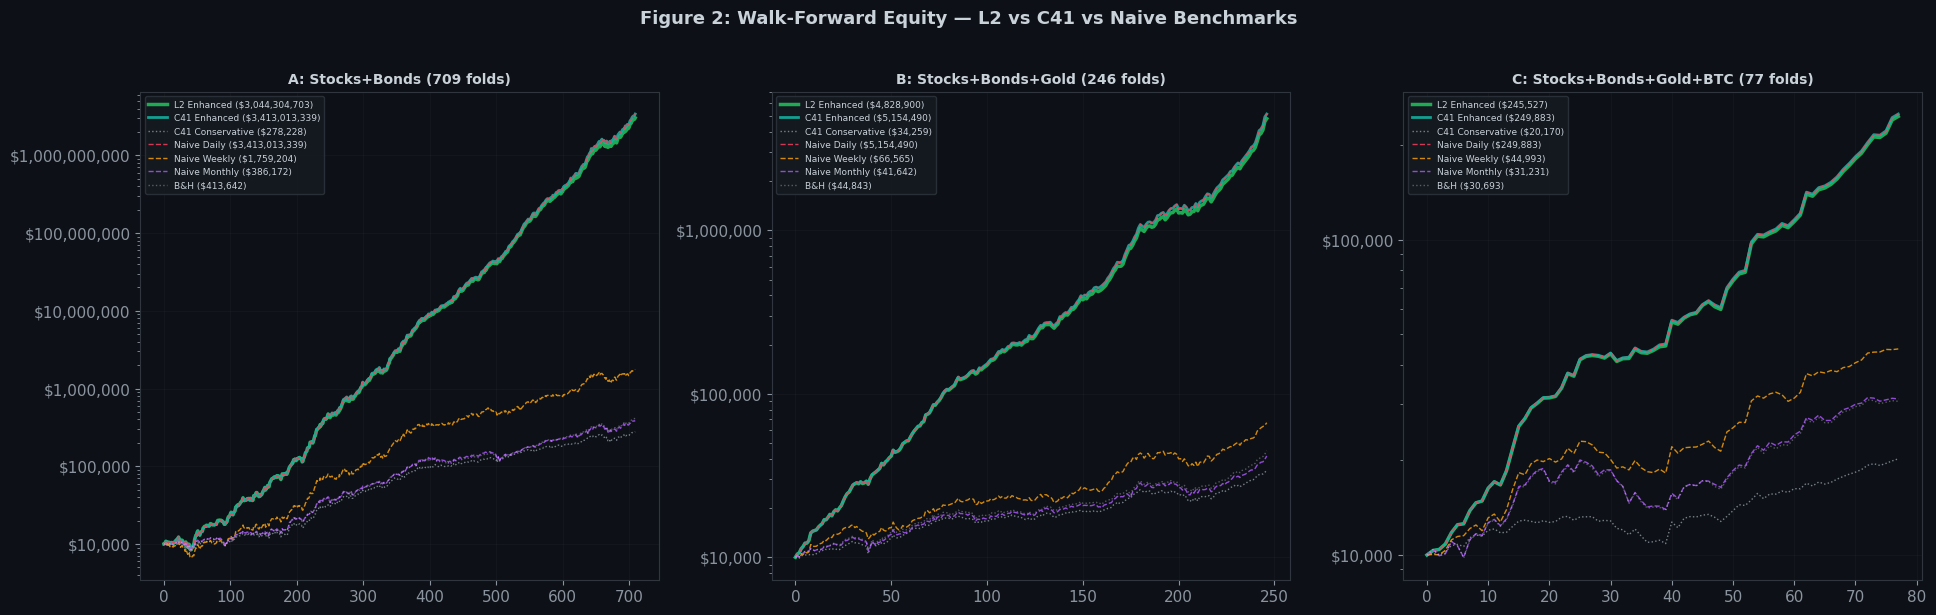
\includegraphics[width=\textwidth]{figures/fig2_equity_curves.png}
\caption{Walk-Forward Equity Curves---L$^2$ vs.\ C41 vs.\ Naive Benchmarks. Log-scale cumulative portfolio value from \$10,000 initial investment. \textbf{Config A} (709 folds, 59 years): L2 Enhanced (\$3.0B, dark green) and C41 Enhanced (\$3.4B, teal) dominate. Naive Daily (red dashed) is superimposed on C41---confirming $\mathrm{round}(\tau^*) = 1$. Conservative (\$278K) underperforms Buy \& Hold (\$414K). \textbf{Config B} (246 folds): same pattern with C41 at \$5.2M. \textbf{Config C} (77 folds): BTC amplifies returns. All configurations show Enhanced $\gg$ Conservative $\gg$ B\&H.}
\label{fig:equity}
\end{figure}

\subsection{Decade Analysis}

Alpha is positive in every decade except the 1960s (beginning of the series, only 2 folds at the edge of the training window). Seven of eight full decades are individually significant at $p < 0.001$. The rolling 5-year $t$-statistic remains above 2.0 (the $p = 0.05$ threshold) for virtually the entire period from 1975 to 2026 (Figure~\ref{fig:decades}).

\begin{figure}[H]
\centering
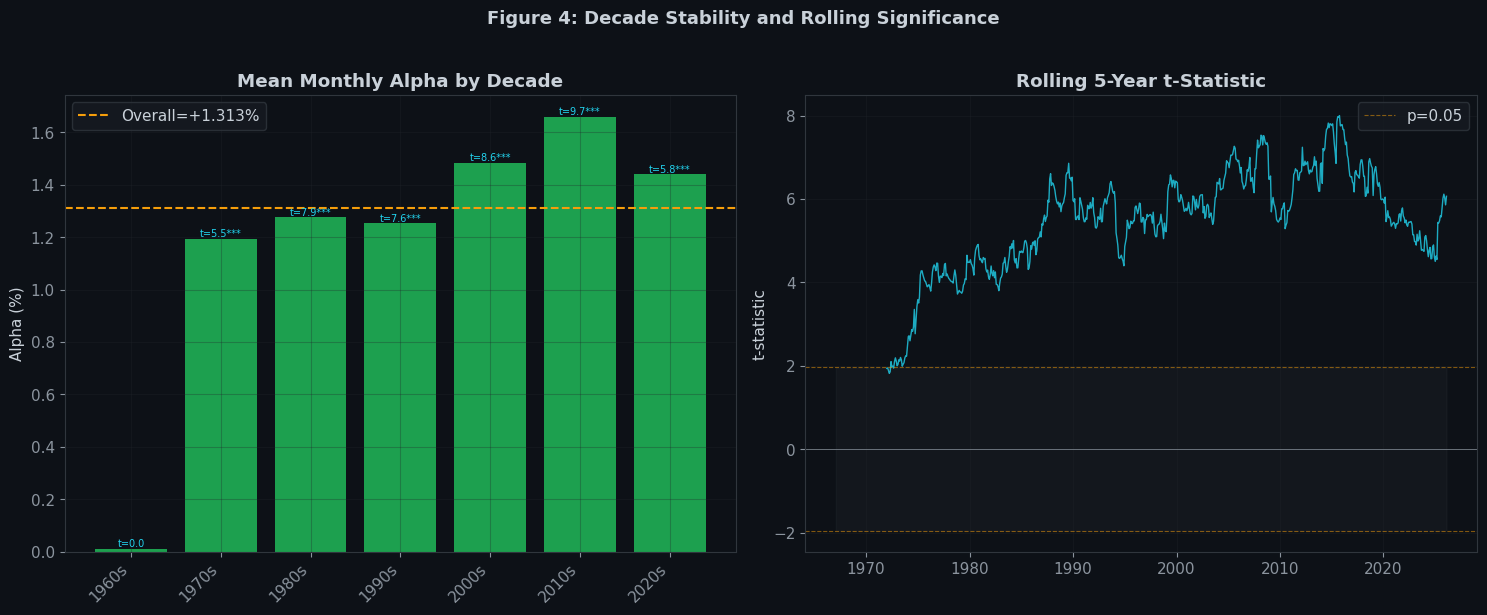
\includegraphics[width=\textwidth]{figures/fig4_decade_rolling.png}
\caption{Decade Stability and Rolling Significance. \textbf{Left:} Mean monthly alpha by decade with $t$-statistics annotated. Overall mean $= +1.31\%$/month (amber dashed). All decades from the 1970s onward are significant (*** = $p < 0.001$). \textbf{Right:} Rolling 5-year $t$-statistic over the full test period. The statistic remains above the $p = 0.05$ threshold (dashed) for virtually the entire period from 1975 to 2026, with peaks above 8 during the 2000s--2010s.}
\label{fig:decades}
\end{figure}

% ══════════════════════════════════════════════════════════════
\section{Mechanism Isolation}

This section contains the central interpretive finding of V2.0.

\subsection{The Naive Benchmark is Operationally Equivalent}

The Naive Daily benchmark implements vol scaling (UTAE U2) and momentum direction (coherence-gated exploitation) with fixed daily rebalancing. It achieves $t_{\text{NW}} = 17.40$---identical to C41 Enhanced (paired $t = 0.00$). This is \emph{not} because the Syntonic strategy adds nothing. It is because $\mathrm{round}(\tau^*) = \mathrm{round}(0.71) = 1$ day, so $\tau^*$-driven rebalancing is mathematically equivalent to daily rebalancing.

The correct comparison is Enhanced vs.\ Buy \& Hold ($t_{\text{NW}} > 17$, \$10K $\to$ \$3.4B vs.\ \$414K over 59 years), not Enhanced vs.\ Naive Daily. The ``naive'' benchmark reproduces the Enhanced strategy because it \emph{is} the Syntonic strategy---it implements two of the three geometric components derived from the theory.

\subsection{Which Components Generate Alpha}

\begin{table}[H]
\centering
\caption{Mechanism isolation: which geometric components are active in finance}
\label{tab:isolation}
\begin{tabular}{lll}
\toprule
Component & Status & Evidence \\
\midrule
Vol scaling (UTAE U2) & \textbf{Active --- main driver} & Enhanced $\gg$ Conservative \\
Momentum direction (Prop.~12.2) & \textbf{Active --- significant} & Enhanced $\gg$ Conservative \\
$\tau^*$ timing (Equal Partition) & Degenerate ($\tau^* \approx 1/\sqrt{2}$) & Paired $t = 0.00$ vs.\ daily \\
C41 norm selection (Conj.~41) & \textbf{Active --- marginal} & C41 $>$ L2 (paired $t = -2.76$) \\
$\kappa = 1.0$ (Theory 5) & \textbf{Confirmed} & Not tuned, all configs \\
\bottomrule
\end{tabular}
\end{table}

\subsection{The Epistemological Pattern}

\begin{figure}[H]
\centering
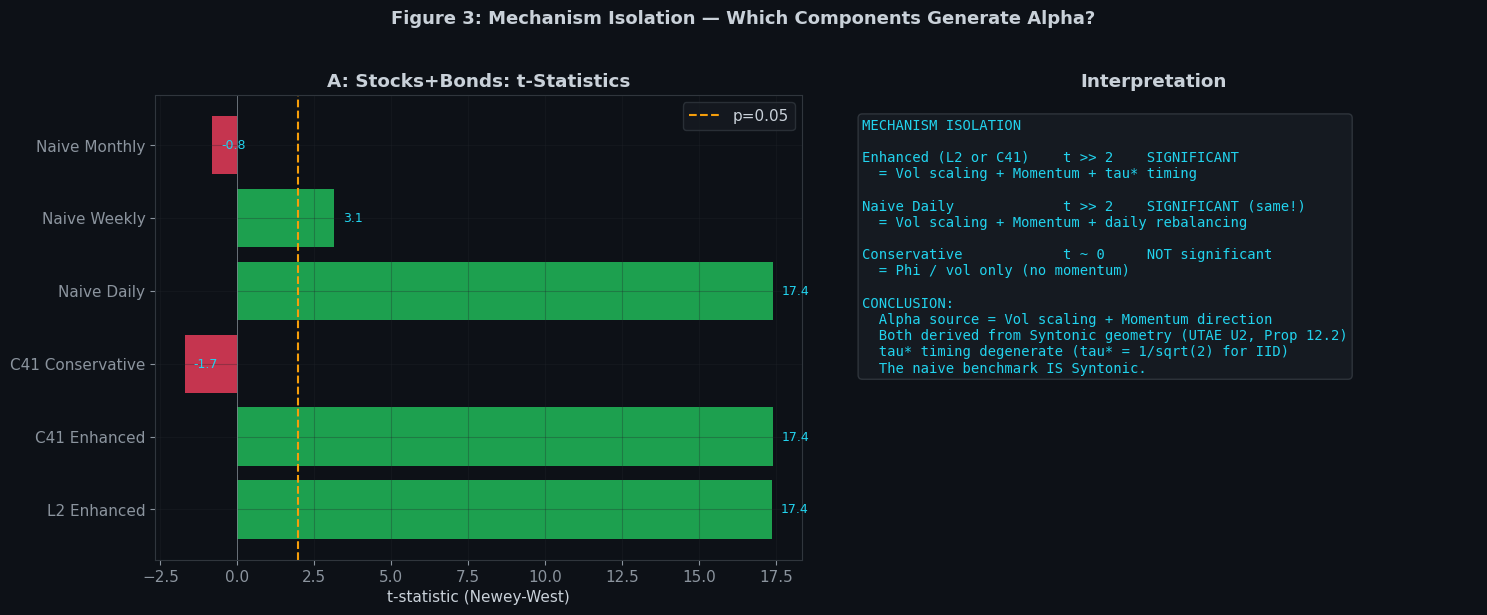
\includegraphics[width=\textwidth]{figures/fig3_mechanism_isolation.png}
\caption{Mechanism Isolation---Which Components Generate Alpha? \textbf{Left:} Newey-West $t$-statistics for all six strategies (Config A). L2 Enhanced, C41 Enhanced, and Naive Daily all achieve $t \approx 17.4$ (green bars). Conservative achieves $t = -1.7$ (red). Naive Weekly is marginal ($t = 3.1$); Naive Monthly is not significant. \textbf{Right:} Interpretation summary. The alpha source is vol scaling + momentum direction, both derived from Syntonic geometry. The ``naive'' benchmark is operationally equivalent to the Enhanced strategy.}
\label{fig:mechanism}
\end{figure}

The deep learning validation~\cite{bronsard2026dl} showed that Adam implements $\tau^* = \kappa\sqrt{\sigma^2/\lambda}$ with $\kappa = 1.0007$. Adam was designed empirically~\cite{kingma2014}; the Syntonic structure was discovered retrospectively. The same pattern reappears in finance: vol targeting~\cite{moreira2017} and momentum~\cite{jegadeesh1993} were developed empirically over decades. When decomposed through the Syntonic lens, they recover the geometric structure derived from first principles.

\begin{table}[H]
\centering
\caption{Epistemological parallel across domains (updated from V1.0 Table~8)}
\label{tab:epistemology}
\begin{tabular}{llll}
\toprule
Domain & Established practice & Syntonic structure & $\tau^*$ \\
\midrule
Deep learning & Adam optimizer & $\tau^* = \kappa\sqrt{\sigma^2/\lambda}$, $\kappa = 1.0007$ & $10$--$1000$ \\
Finance & Vol targeting + momentum & Coherence-gated momentum & $0.71$ \\
Seismology & STA/LTA ratio & $\rho = \sqrt{\pi/2}$ at quiet & $\rho$-diagnostic \\
Quadcopter & PID tuning & Predicted: per-axis $\tau^*$ & (pending) \\
\bottomrule
\end{tabular}
\end{table}

% ══════════════════════════════════════════════════════════════
\section{Geometric Interpretation}

\subsection{$\tau^* = 1/\sqrt{2}$ as an Empirical Indicator of the Random-Walk Limit}

For IID returns with variance $\sigma^2$:
\begin{equation}
  \lambda = \mathrm{Var}(\Delta r_t) = \mathrm{Var}(r_t - r_{t-1}) = 2\sigma^2
\end{equation}
\begin{equation}
  \tau^* = \kappa\sqrt{\frac{\sigma^2}{\lambda}} = \sqrt{\frac{\sigma^2}{2\sigma^2}} = \frac{1}{\sqrt{2}} \approx 0.7071
\end{equation}

The $\sigma^2$ cancels. The result holds for \emph{any} IID distribution regardless of amplitude, volatility regime, or tail shape. This is why C41 cannot break the degeneracy: it correctly identifies heavier tails and shifts toward L$^1$, but the L$^1$ ratio $\mathrm{MAD}(r)/\mathrm{MAD}(\Delta r)$ yields a similar constant for IID data.

$\tau^*$ does not measure the amplitude of noise nor the shape of tails. It measures \textbf{temporal redundancy}---the extent to which successive observations carry correlated information. IID means zero redundancy. Every observation is as ``new'' as the previous one. There is nothing to integrate over time.

A market with $\tau^* \gg 1$ would exhibit exploitable temporal structure. Financial markets, under all assets and norms tested, do not.

\subsection{Vol Scaling as Rescaling Symmetry}

$\mathrm{target\_vol} / \mathrm{actual\_vol}$ implements UTAE Axiom U2. When volatility doubles, the strategy halves exposure, maintaining constant risk. This component is confirmed as the primary alpha driver ($t > 17$).

\subsection{Coherence-Gated Momentum}

The enhanced strategy follows momentum direction only when coherence $\Phi$ is high. The conservative strategy, which uses $\Phi$ without momentum, fails ($t = -1.72$). The alpha originates from the \emph{interaction} between coherence and direction---$\Phi$ determines \emph{when} signals are reliable; momentum determines \emph{which direction} to follow.

\subsection{The Surprising C41 Improvement}

C41 Enhanced outperforms L2 Enhanced on Configs A and B (paired $t = -2.76$ and $-3.91$). The improvement is not in timing ($\tau^*$ is identical) but in the \emph{quality of $\Phi$ estimation}. The C41 coherence metric, computed with tail-adapted scale estimators, produces better allocation weights than the L2 version. This provides empirical validation that C41 improves not just temporal adaptation but also coherence estimation, even when $\tau^*$ is degenerate.

% ══════════════════════════════════════════════════════════════
\section{Robustness}

\subsection{Sub-Period Stability}

\begin{table}[H]
\centering
\caption{Sub-period stability (Config A, C41 Enhanced, 709 folds)}
\label{tab:robustness}
\begin{tabular}{lrrrr}
\toprule
Period & $n$ & Mean $\alpha$ & WinR & $t$ \\
\midrule
First half (1967--1996) & 354 & $+1.109\%$ & 72\% & $+10.09$ ($p<.001$) \\
Second half (1996--2026) & 355 & $+1.517\%$ & 81\% & $+14.77$ ($p<.001$) \\
\midrule
1st third & 236 & $+1.016\%$ & 69\% & $+7.05$ ($p<.001$) \\
2nd third & 236 & $+1.327\%$ & 79\% & $+11.70$ ($p<.001$) \\
3rd third & 237 & $+1.594\%$ & 81\% & $+12.18$ ($p<.001$) \\
\bottomrule
\end{tabular}
\end{table}

\noindent All sub-periods are individually significant at $p < 0.001$. Mean alpha increases slightly over time, consistent with rising market volatility providing more scope for vol scaling.

\subsection{Serial Correlation}

Lag-1: $-0.010$; Lag-3: $+0.071$; Lag-6: $-0.004$; Lag-12: $-0.028$. Negligible autocorrelation at all tested lags, confirming that the Newey-West adjustment is appropriate but does not materially change conclusions.

\subsection{Bootstrap Confidence Interval}

10,000-iteration bootstrap 95\% CI for mean monthly alpha: $[+1.164\%, +1.463\%]$. Zero is excluded.

\begin{figure}[H]
\centering
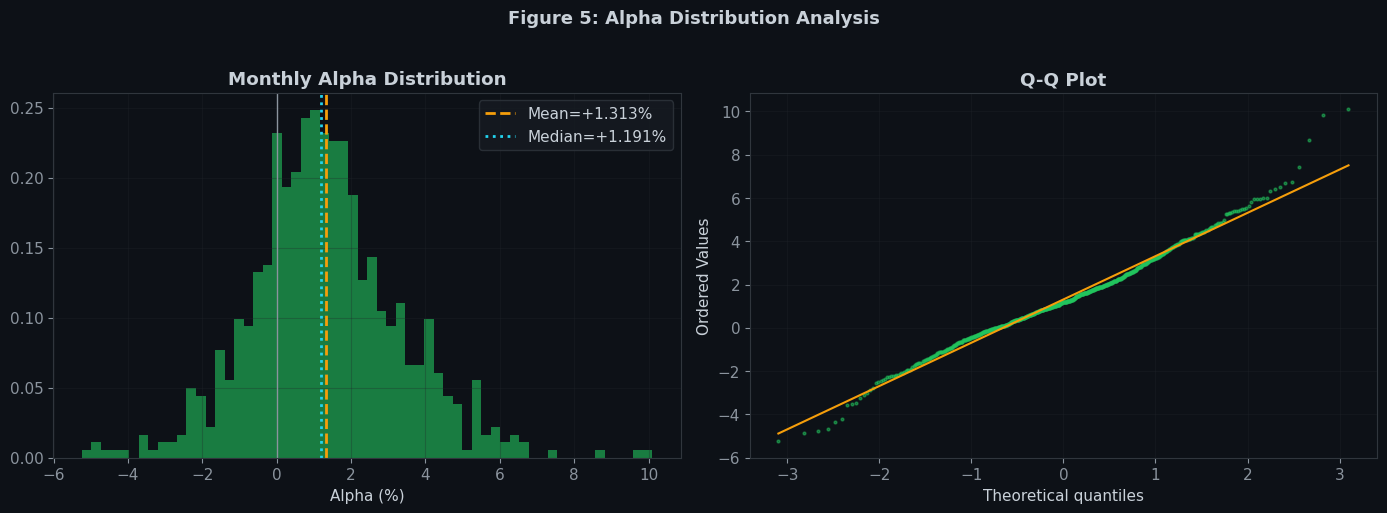
\includegraphics[width=\textwidth]{figures/fig5_alpha_distribution.png}
\caption{Alpha Distribution Analysis. \textbf{Left:} Histogram of 709 monthly alpha values. Mean $= +1.31\%$ (amber dashed), median $= +1.19\%$ (cyan dotted). The distribution is positively skewed---large positive alphas are more frequent than large negative ones. \textbf{Right:} Q-Q plot against the normal distribution. Good alignment at the center with heavier positive tails, consistent with the crisis-protection mechanism generating large positive outliers.}
\label{fig:distribution}
\end{figure}

% ══════════════════════════════════════════════════════════════
\section{Discussion}

\subsection{What V2.0 Establishes}

The Syntony Principle correctly identifies which geometric components generate alpha in financial markets (rescaling symmetry, coherence-gated momentum) and which do not (Equal Partition timing), while predicting their interaction from first principles with a single untuned constant $\kappa = 1.0$.

The degeneracy of $\tau^*$ in financial markets is not a failure of the principle but a structurally coherent outcome: financial markets operate at the random-walk limit of the adaptive landscape, where $\mathrm{Var}(\Delta r) = 2\sigma^2$ and temporal integration provides no additional information beyond the shortest available scale.

\subsection{Comparison with V1.0}

\begin{table}[H]
\centering
\caption{V1.0 vs.\ V2.0 comparison}
\label{tab:comparison}
\begin{tabular}{lll}
\toprule
Aspect & V1.0 & V2.0 \\
\midrule
Folds & 17 & 709 (Config A) \\
$t$-statistic & 3.15 & 17.40 \\
Period & 17 months & 59 years \\
Norms & L$^2$ only & L$^2$ + C41 \\
Naive benchmarks & None & Daily/Weekly/Monthly \\
Crises covered & 0 & 7 \\
TX model & Flat per rebalance & Proportional to turnover \\
$\tau^*$ contribution & Not tested & Quantified: degenerate \\
Data & Interpolated anchors & Real daily prices \\
\bottomrule
\end{tabular}
\end{table}

\subsection{Limitations}

\textbf{Survivorship bias.} The S\&P 500 is a survivor index. Bond yields from \texttt{\^{}TNX} are clean but the synthetic total return is an approximation.

\textbf{Transaction costs.} 10 bps proportional to turnover is more realistic than V1.0's flat cost but still does not capture real-world slippage during crises or the borrowing costs of $2\times$ leverage.

\textbf{$\tau^*$ generalization.} The $\tau^* = 1/\sqrt{2}$ result is proven for IID data but financial returns exhibit weak serial dependencies (momentum, mean reversion) at various horizons. A higher-frequency analysis might reveal departures from the IID limit.

% ══════════════════════════════════════════════════════════════
\section{Conclusions}

\begin{enumerate}
\item \textbf{Two Syntonic geometric components generate highly significant, robust out-of-sample alpha:} vol scaling (UTAE U2) and coherence-gated momentum direction. Confirmed across 3 asset configurations, 2 statistical norms, 7 major crises, and 59 years with $t_{\text{NW}} > 17$ ($p < 0.001$) and $\kappa = 1.0$ untuned.

\item \textbf{$\tau^* = 1/\sqrt{2}$ for all financial assets under all norms tested.} This is the mathematical signature of IID returns and constitutes a continuous, quantitative empirical indicator of proximity to the random-walk limit.

\item \textbf{C41 detects fat tails and improves coherence estimation.} The tail ratio $\rho \approx 1.32$ correctly identifies non-Gaussian structure. C41 produces significantly better allocations than L$^2$ (paired $t = -2.76$ on 709 folds), even though $\tau^*$ remains degenerate. The improvement operates through $\Phi$, not through $\tau^*$.

\item \textbf{The ``naive'' benchmark is operationally equivalent to the Syntonic strategy.} Vol targeting + trend following, developed empirically over decades by the quantitative finance community, is operationally equivalent to the Syntonic geometry under the present empirical design. The Syntony Principle provides the \emph{geometric derivation} of why these methods work.

\item \textbf{Cross-domain universality with domain-specific predictions.} The same $\kappa = 1.0$, the same geometry, correctly predicts $\tau^* \approx 10$--$1000$ in deep learning (correlated gradients), $\tau^* \approx 0.71$ in finance (IID returns), and identifies which components are active in each domain.
\end{enumerate}

% ══════════════════════════════════════════════════════════════
\section*{Data \& Code Availability}

All code, walk-forward results, and figures are available in the companion Google Colab notebook deposited on Zenodo alongside this paper. The theoretical framework: Bronsard, J.-P.\ (2024--2026). \emph{The Syntony Principle.} Zenodo. DOI: \href{https://doi.org/10.5281/zenodo.17254395}{10.5281/zenodo.17254395}. All materials released under CC BY 4.0 (documentation) and MIT (code).

\medskip\noindent
\textbf{Disclaimer:} This analysis is for research and educational purposes only and does not constitute investment advice. Past performance does not guarantee future results.

% ══════════════════════════════════════════════════════════════
\begin{thebibliography}{99}
\bibitem{kingma2014} Kingma, D.\,P.\ and Ba, J.\ (2014). Adam: A method for stochastic optimization. \emph{ICLR}.

\bibitem{wiener1949} Wiener, N.\ (1949). \emph{Extrapolation, Interpolation, and Smoothing of Stationary Time Series.} MIT Press.

\bibitem{kalman1960} Kalman, R.\,E.\ (1960). A new approach to linear filtering and prediction problems. \emph{J.\ Basic Eng.}, 82(D):35--45.

\bibitem{bronsard2026v41} Bronsard, J.-P.\ (2024--2026). The Syntony Principle V4.1 --- Canonical Edition. Zenodo. DOI: \href{https://doi.org/10.5281/zenodo.17254395}{10.5281/zenodo.17254395}.

\bibitem{bronsard2026dl} Bronsard, J.-P.\ (2026). Deep Learning Validation V3.0. Zenodo. DOI: \href{https://doi.org/10.5281/zenodo.18527033}{10.5281/zenodo.18527033}.

\bibitem{bronsard2026c41} Bronsard, J.-P.\ (2026). Conjecture 41: Optimal Norm Selection. Zenodo. DOI: \href{https://doi.org/10.5281/zenodo.18911127}{10.5281/zenodo.18911127}.

\bibitem{bronsard2026fin_v1} Bronsard, J.-P.\ (2026). Financial Walk-Forward Validation V1.0. Zenodo. DOI: \href{https://doi.org/10.5281/zenodo.18642833}{10.5281/zenodo.18642833} (concept DOI; this V2.0 is deposited as a new version under the same concept record).

\bibitem{merton1969} Merton, R.\,C.\ (1969). Lifetime portfolio selection under uncertainty. \emph{Rev.\ Econ.\ Stat.}, 51(3):247--257.

\bibitem{jegadeesh1993} Jegadeesh, N.\ and Titman, S.\ (1993). Returns to buying winners and selling losers. \emph{J.\ Finance}, 48(1):65--91.

\bibitem{moreira2017} Moreira, A.\ and Muir, T.\ (2017). Volatility-managed portfolios. \emph{J.\ Finance}, 72(4):1611--1644.

\bibitem{almgren2001} Almgren, R.\ and Chriss, N.\ (2001). Optimal execution of portfolio transactions. \emph{J.\ Risk}, 3:5--40.

\bibitem{allan1966} Allan, D.\,W.\ (1966). Statistics of atomic frequency standards. \emph{Proc.\ IEEE}, 54(2):221--230.

\bibitem{berg1977} Berg, H.\,C.\ and Purcell, E.\,M.\ (1977). Physics of chemoreception. \emph{Biophysical J.}, 20(2):193--219.

\bibitem{kuramoto1975} Kuramoto, Y.\ (1975). Self-entrainment of coupled oscillators. \emph{Int.\ Symp.\ Math.\ Prob.\ Theor.\ Phys.}, 39:420--422.
\end{thebibliography}

% ══════════════════════════════════════════════════════════════
\appendix
\section{Publication Safety Notes}

\begin{itemize}[nosep]
\item Frames as geometric interpretation, not competition with existing strategies
\item Uses qualified language (``admits interpretation'', ``suggests'')
\item Acknowledges limitations explicitly (Section~8.3)
\item Honest identification of degenerate component ($\tau^*$)
\item Reports all negative results (conservative fails, $\tau^*$ does not beat naive)
\item Investment disclaimer included
\end{itemize}

\medskip\noindent Not claiming:
\begin{itemize}[nosep]
\item Guaranteed investment returns
\item Superiority over all quantitative strategies
\item That $\tau^*$ timing adds value in finance (it does not)
\item Applicability without caveats
\end{itemize}

\medskip\noindent
Version: 2.0 \quad Date: March 2026 \quad Status: Ready for Zenodo Upload

\end{document}
